\section{Grafički prikazi}

U nastavku su prikazane različite grafičke reprezentacije podataka kako bi se dobila bolja vizualna interpretacija distribucije.

\begin{figure}[H]
\centering
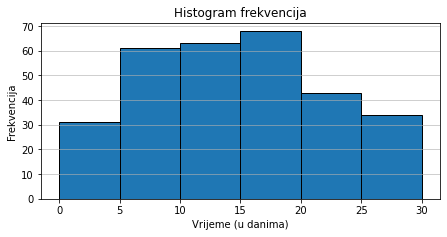
\includegraphics[width=1\textwidth]{assets/histogram_frekvencija.png}
\caption{Histogram frekvencija}
\end{figure}

\begin{figure}[H]
\centering
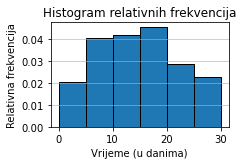
\includegraphics[width=1\textwidth]{assets/histogram_relativnih_frekvencija.png}
\caption{Histogram relativnih frekvencija}
\end{figure}

\begin{figure}[H]
\centering
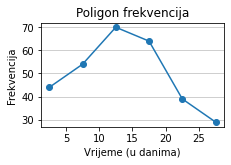
\includegraphics[width=0.9\textwidth]{assets/poligon_frekvencija.png}
\caption{Poligon frekvencija}
\end{figure}

\begin{figure}[H]
\centering
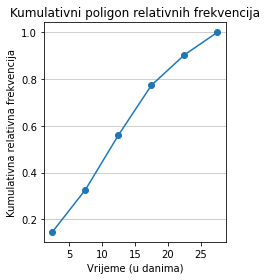
\includegraphics[width=0.7\textwidth]{assets/kumulativni_poligon_relativnih_frekvencija.png}
\caption{Kumulativni poligon relativnih frekvencija}
\end{figure}

\begin{figure}[H]
\centering
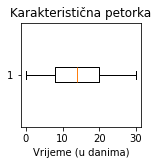
\includegraphics[width=0.5\textwidth]{assets/karakteristicna_petorka.png}
\caption{Karakteristična petorka, prikazana kutijastim dijagramom tzv. \textit{box plot}}
\end{figure}

\begin{figure}[H]
\centering
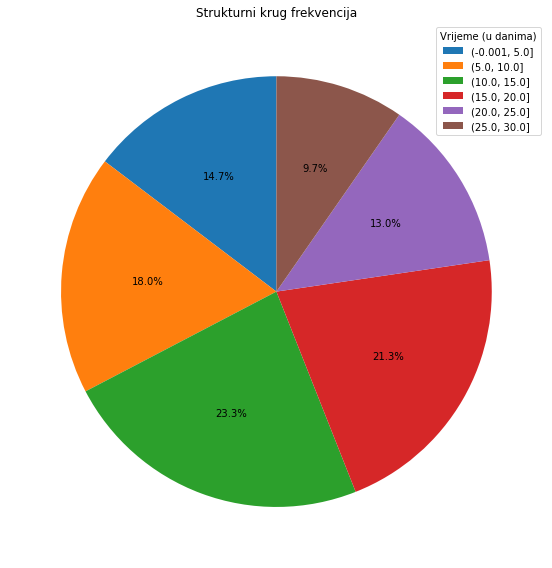
\includegraphics[width=0.8\textwidth]{assets/strukturni_krug_frekvencija.png}
\caption{Strukturni krug frekvencija, prikazan kružnim dijagramom tzv. \textit{pie chart}}
\end{figure}

\newpage

U ispisu~\ref{graphics} prikazan je način na koji je bilo potrebno konfigurirati i postaviti \textit{plot} iz biblioteke \texttt{matplotlib} kako bi se što jasnije prethodno izračunate vrijednosti grafički prikazale te k\^od koji je zaslužan za crtanje svakog od prikazanih grafikona.

\begin{lstlisting}[caption={Način konstruiranja grafičkih prikaza koristeći biblioteku \texttt{matplotlib}}, label=graphics]
# Racunanje sredisnjih tocki za iscrtavanje na grafu
midpoints = [interval.mid for interval in frequency_table.index]

plt.subplot(2, 2, 1)
plt.hist(data['Vrijeme'], bins=bins, edgecolor='black')
plt.title('Histogram frekvencija')
plt.xlabel('Vrijeme (u danima)')
plt.ylabel('Frekvencija')
plt.grid(axis='y', alpha=0.75)
plt.tight_layout()
plt.show()

plt.subplot(2, 2, 2)
plt.hist(data['Vrijeme'], bins=bins, density=True, edgecolor='black')
plt.title('Histogram relativnih frekvencija')
plt.xlabel('Vrijeme (u danima)')
plt.ylabel('Relativna frekvencija')
plt.grid(axis='y', alpha=0.75)
plt.tight_layout()
plt.show()

plt.subplot(2, 2, 3)
plt.plot(midpoints, frequency_table.values, marker='o')
plt.title('Poligon frekvencija')
plt.xlabel('Vrijeme (u danima)')
plt.ylabel('Frekvencija')
plt.grid(axis='y', alpha=0.75)
plt.tight_layout()
plt.show()

plt.subplot(1, 2, 1)
plt.plot(midpoints, cumulative_relative_frequency.values, marker='o')
plt.title('Kumulativni poligon relativnih frekvencija')
plt.xlabel('Vrijeme (u danima)')
plt.ylabel('Kumulativna relativna frekvencija')
plt.grid(axis='y', alpha=0.75)
plt.tight_layout()
plt.show()

plt.subplot(2, 3, 6)
plt.boxplot(data['Vrijeme'], vert=False)
plt.title('Karakteristicna petorka')
plt.xlabel('Vrijeme (u danima)')
plt.tight_layout()
plt.show()

plt.figure(figsize=(8, 8))
wedges, texts, autotexts = plt.pie(frequency_table, autopct='%1.1f%%', startangle=90)
plt.title('Strukturni krug frekvencija')
plt.legend(wedges, frequency_table.index, title='Vrijeme (u danima)')
plt.tight_layout()
plt.show()
\end{lstlisting}